\section{Electromagnetic fields in Media II}

\subsection{Review}
Last time we reviewed notions of EM in media in the static case as you learned last quarter. We made a couple approximations; first we assumed a linear relationship between the polarization and the electric field:
\begin{equation}
    \avg{\v{P}}(t, \v{x}) = \e_0 \chi \avg{\v{E}}(t, \v{x})
\end{equation}
where $\avg{\cdot}$ denotes averaging over region of macroscopic size $L$. The above equation is equivalent to:
\begin{equation}
    \avg{\v{D}}(t, \v{x}) = \e\avg{\v{E}}(t, \v{x})
\end{equation}
Two curious things - the polarization is sensitive instantaneously at time $t$, and it is also local in $\v{x}$. The second observation is ok (in the non-relativistic setting), but the first is a bit concerning - we would expect the polarization in the material to be resulting from the electric field at some earlier time; different effects/influences take time to propagate in the material. So, we should refine the causality in the above formulas.

\subsection{Refinement of Polarization Formula}
A more realistic model would have that $\avg{\v{P}}(t, \v{x})$ can be influenced by $\avg{\v{E}}(t', \v{x})$ with $t' < t$. This effect should (for small enough $\v{E}$) only depend on $t - t'$. In particular:

\begin{equation}
    \avg{\v{P}}(t, \v{x}) = \int_{-\infty}^\infty dt' f(t - t')\avg{\v{E}}(t', \v{x})
\end{equation}

with an example of $f$ sketched below; it is $0$ for $t' > t$ goes to 0 rapidly as $t - t' \to \infty$. 

\begin{center}
    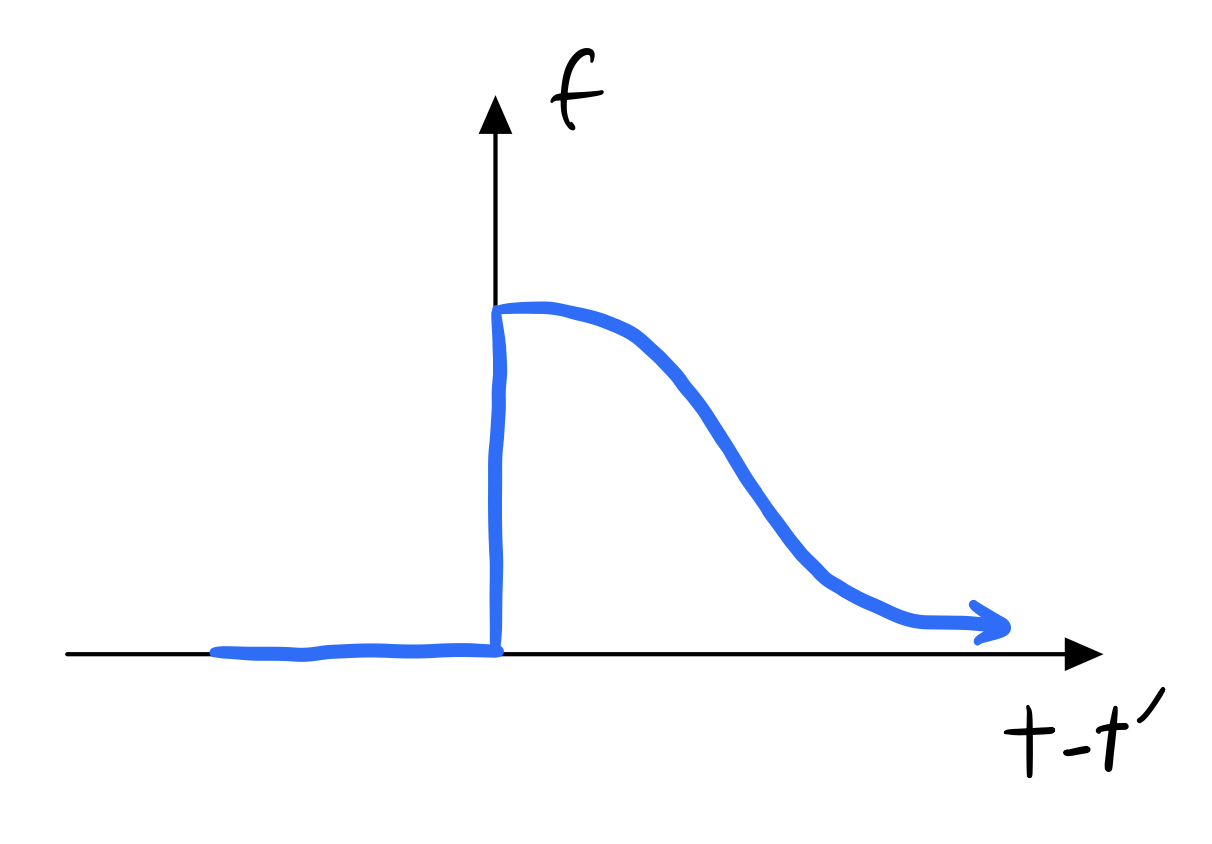
\includegraphics[scale=0.35]{Lectures/Images/lec13-ffunction.png}
\end{center}


It will be helpful to fourier transform in time:
\begin{equation}
    \avg{\tilde{\v{P}}}(\omega) = \frac{1}{\sqrt{2\pi}}\int_{-\infty}^\infty e^{i\omega t}\avg{\v{P}}(t) = \sqrt{2\pi}\tilde{f}(\omega)\avg{\tilde{\v{E}}}(\omega)
\end{equation}
where we use that a fourier transform of a convolution leads to a product, and $\tilde{f}(\omega)$ is:
\begin{equation}\label{eq:fomega}
    \tilde{f}(\omega) = \frac{1}{\sqrt{2\pi}}\int_{-\infty}^\infty dt e^{i\omega t}f(t)
\end{equation}
In our old/causally incorrect formula, we took $f(t - t') = \delta(t - t')$ in which case $\tilde{f}(\omega)$ is a constant. In our more interesting/sophsticated model, we have that:
\begin{equation}
    \avg{\tilde{\v{P}}}(\omega) = \e_0 \chi(\omega)\avg{\tilde{\v{E}}}(\omega)
\end{equation}
where the susceptibility takes on a frequency dependence:
\begin{equation}
    \chi(\omega) = \frac{\sqrt{2\pi}}{\e_0}\tilde{f}(\omega)
\end{equation}
and similarly for the permittivity we have:
\begin{equation}
    \avg{\tilde{\v{D}}}(\omega) = \e(\omega)\avg{\tilde{\v{E}}}(\omega)
\end{equation}
with:
\begin{equation}
    \e(\omega) = \e_0(1 + \chi(\omega))
\end{equation}
And further similarly we have for the magnetic field that:
\begin{equation}
    \avg{\tilde{\v{H}}}(\omega) = \frac{1}{\mu(\omega)}\avg{\tilde{\v{B}}}(\omega)
\end{equation}

\subsection{Complex frequencies and Kramers-Kronig Relations}
We can now ask - what happens if we take $\omega$ to be complex. This may sound like a ridiculous question, but in fact this will have very physical consequences. Suppose $\Im(\omega) > 0$ such that:
\begin{equation}
    \omega = \omega_1 + i\omega_2
\end{equation}
with $\omega_2 > 0$. We restrict our attention to the upper half of the complex plane. Then what happens? If we plug this into our formula in Eq. \eqref{eq:fomega}, we get the oscillating part $e^{i\omega_1 t}$ from $\omega_1$ and a real exponential $e^{-\omega_2 t}$ from $\omega_2$. This goes to 0 as $t \to \infty$ - it might be a priori concerning, but then we recall that our function $f$ is 0 when its argument is negative ($f(x < 0) = 0$) which means that $\tilde{f}(\omega)$ is convergent in the UHP. Furthermore, it is a holomorphic function. In your problem set, you will derive the Kramers-Kronig relations (for the real/part of the susceptibility):
\begin{equation}
    \Re\chi(\omega) = \frac{1}{\pi}\mathbb{P}\int_{-\infty}^\infty d\omega' \frac{\Im(\chi(\omega'))}{\omega' - \omega}
\end{equation}
\begin{equation}
    \Im\chi(\omega) = -\frac{1}{\pi}\mathbb{P}\int_{-\infty}^\infty d\omega' \frac{\Re(\chi(\omega'))}{\omega' - \omega}
\end{equation}
What is the $\mathbb{P}$ appearing in the above? It denotes that we take the principle value of the integrals. We break up the integration region, remove a region of size $\e$ around $\omega$ to avoid the singularity, and then take $\e \to 0$ in the end.

\begin{center}
    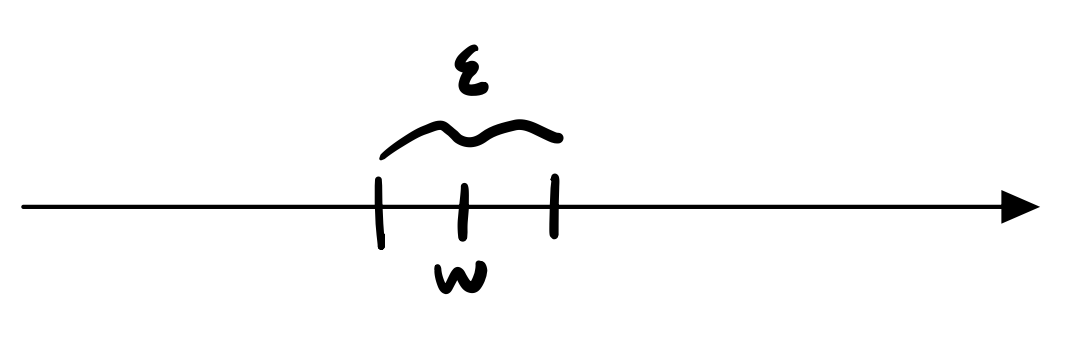
\includegraphics[scale=0.35]{Lectures/Images/lec13-principal.png}
\end{center}

A remark - taking the complex conjugate of \eqref{eq:fomega} we find:
\begin{equation}
    \tilde{f}^*(\omega) = \frac{1}{\sqrt{2\pi}}\int_{-\infty}^\infty dt e^{-i\omega t}f(t)
\end{equation}
where $f^*(t) = f(t)$ as it is real. Hence:
\begin{equation}
    \tilde{f}^*(\omega) = \tilde{f}(-\omega)
\end{equation}
Thus:
\begin{equation}
    \chi^*(\omega) = \chi(-\omega)
\end{equation}
and hence we may rewrite the Kramers-Kronig relations to be:
\begin{equation}
    \Re \chi(\omega) = \frac{2}{\pi}\mathbb{P}\int_0^\infty d\omega' \frac{\Im(\chi(\omega'))\omega'}{\omega'^2 - \omega^2}
\end{equation}
\begin{equation}
    \Im \chi(\omega) = -\frac{2\omega}{\pi}\mathbb{P}\int_0^\infty d\omega' \frac{\Re(\chi(\omega'))\omega'}{\omega'^2 - \omega^2}
\end{equation}

\subsection{Absorption and Complex Indices of Refraction}
This seems like something that maybe only someone in Eckhart would enjoy, but indeed this is a very useful notion for people that actually build things with screwdrivers and work with materials etc. We first note that $\chi(\omega)$ cannot be real. Indeed, if it is the case that $\Im\chi(\omega) = 0$, then $\Re\chi(\omega) = 0$ by the Kramers-Kronig relation. What implication does this have for electromagnetic wave propagation in materials? Indeed, the index of refraction:
\begin{equation}
    n(\omega) = c\sqrt{\e(\omega)\mu(\omega)}
\end{equation}
becomes complex, as $\e(\omega)$ has an imaginary part (assuming $\mu(\omega)$ does not cancel this out). This implies that EM waves are absorbed in material - they don't just purely propagate! Indeed, if we have a wave $e^{-i\omega t + ikx}$ with $k = \frac{\omega}{c(\omega)} = \frac{\omega}{\frac{c}{n(\omega)}} = k_1 + ik_2$, and our above argument tells us that $k_2 \neq 0$, so in addition to have a spatially oscillating part $e^{ik_1 x}$ we also have an exponentially decaying part $e^{-ik_2 x} = e^{-\gamma x}$ (one could argue that depending on the sign of $\gamma$ we could have exponential amplification instead, but it can't possibly be that the amplitude gets arbitrarily amplified in a material, so it must be that $\gamma > 0$). Not only can we qualitatively conclude that there is absorption, we can calculate it explicitly. It is worth noting that this effect is generally quite small (e.g. for things like glass) so $e^{-\gamma x} \sim 1$ (and this is the limit in which optical laws such as Snell's law are derived).

\subsection{Phase and Group Velocities}
Recall:
\begin{equation}
    v_p = \frac{\omega}{k} = \frac{c}{n(\omega)}
\end{equation}
\begin{equation}
    v_g = \dod{\omega}{k}
\end{equation}
We again consider a plane wave $e^{-i(\omega t - \v{k} \cdot \v{x})}$ with $\omega = \frac{c}{n(\omega)}k$. A surface of fixed phase - $\omega t - \v{k} \cdot \v{x} = \text{const}$ propagates with velocity $v_p = \frac{c}{n(\omega)}$. On the other hand, if we have a wavepacket:
\begin{equation}
    \psi(t, z) = \int dk F(k)e^{-i(\omega t - kz)}
\end{equation}
which is sharply peaked around $k = k_0$:

\begin{center}
    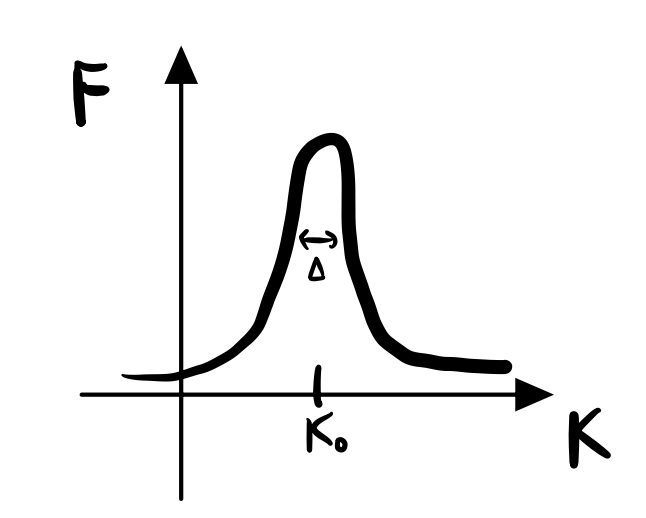
\includegraphics[scale=0.35]{Lectures/Images/lec13-peaked.png}
\end{center}

We Taylor expand $\omega(k)$ around $k_0$:
\begin{equation}
    \omega(k) = \omega(k_0) + (k- k_0)\left.\dod{\omega}{k}\right|_{k_0} + \ldots
\end{equation}
and in the limit of small $\Delta$ we may neglect the subleading terms. Plugging this into our expression for $\psi$:
\begin{equation}
    \psi(t, z) =  \int dk F(k)e^{-i((\omega(k_0) - (k-k_0)\od{\omega}{k}(k_0))t - kz)} = e^{-i(\omega(k_0)t - k_0z)}\int F(k)e^{-i(k - k_0)(\left.\od{\omega}{k}\right|_{k_0}t - z)}dk = e^{-ik_0(v_p t - z)}F(v_g t - z)
\end{equation}
So we can see the wavepacket itself travells with group velocity $v_g$. Let's compute this:
\begin{equation}
    v_g = \dod{\omega}{k} = \left(\dod{k}{\omega}\right)^{-1} = \left(\dod{}{k}(\frac{1}{c}\omega n(\omega))\right)^{-1} = \frac{c}{n + \omega\od{n}{\omega}}
\end{equation}
Where the $\omega \od{n}{\omega}$ contribution can make the group velocity differ from the phase velocity.

Note that if $n(\omega) < 1$, then $v_p > c$. How does this not violate the idea of causality? Well, the bound of causality is set by the fact that if we set initial conditions at some point, then they can only influence things within the causal lightcone (bounded by the speed of light). But plane waves permeate through all space through all time, and there is no information contained in the wave - so there is no a priori reason why the phase velocity needs to be bounded by the speed of light.

\subsection{Lorentz Model for $\e(\omega)$}
This is a particularly simple model for the permittivity of a material - it isn't perfect, but can give us some intuition. Consider a case where we have no free charges/currents and the permeability has no frequency dependence:
\begin{equation}
    \avg{\rho_f} = 0
\end{equation}
\begin{equation}
    \avg{\v{J}_f} = 0
\end{equation}
\begin{equation}
    \mu(\omega) = \mu_0
\end{equation}
so the star of the show is $\e(\omega)$. What happens when we hit the material with an oscillating E/B field? The electrons in the material act as an oscillator.

\begin{center}
    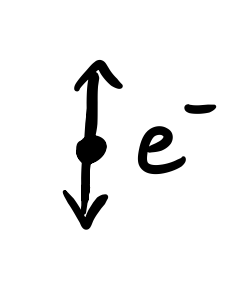
\includegraphics[scale=0.35]{Lectures/Images/lec13-oscillatinge.png}
\end{center}

So let us write their equation of motion as:
\begin{equation}
    m\ddot{\v{x}} + m\gamma \dot{\v{x}} + m\omega_0^2(\v{x} - \v{x}_0') = e\v{E}
\end{equation}
where $\gamma$ is the damping, $\omega_0$ is the natural oscillation frequency of the electron, and $\v{x}_0'$ is the equilibrium position. We use this model to consider three cases:
\begin{enumerate}
    \item \emph{Non-conducting medium.} In this case $\omega_0^2 > 0$ as the electrons experience a restoring force.
    \item \emph{Plasma.} In this case there is no restoring force (electrons are free to propagate), so $\omega_0^2 = 0$, but we do have damping, so $\gamma > 0$.
    \item \emph{Conductors.} In this case, we have unbound electrons with $\omega_0^2 = 0$ and bound electrons with $\omega_0^2 > 0$.
\end{enumerate}

Next time we continue to study this model - it's quite primitive, say, compared to what you may study in a condensed matter course, but it will give us some intuition about the EM response of materials.